\documentclass[onecolumn, 11pt, a4paper]{article}
\usepackage[a4paper, left = 1cm,right = 1cm, top = 1cm, bottom = 1cm, footskip = 0.5cm]{geometry}
% \usepackage{pgfplots}
% \usepackage{physics}
% \usepackage{amsmath}
\usepackage{graphicx}
\usepackage{subfig}
\usepackage{float}
% \usepackage{titlesec}
 
\graphicspath{{./images/}}
% \pgfplotsset{compat = 1.17}

% \titlespacing\section{0pt}{12pt plus 4pt minus 2pt}{0pt plus 2pt minus 2pt}
% \titlespacing\subsection{0pt}{12pt plus 4pt minus 2pt}{0pt plus 2pt minus 2pt}

\author{
  % George Herbert\\
  % \texttt{cj19328@bristol.ac.uk}
}
\date{}

\title{\vspace{-2em}No Entry Sign Challenge Report\vspace{-2em}}

\begin{document}

\maketitle

% \begin{abstract}
%     Abstract
% \end{abstract}

\section{The Viola-Jones object detector}

\subsection{Ground truth and visualisation}

\begin{figure}[H]
  \vspace{-2em}
  \centering
  \subfloat[NoEntry1.jpg]{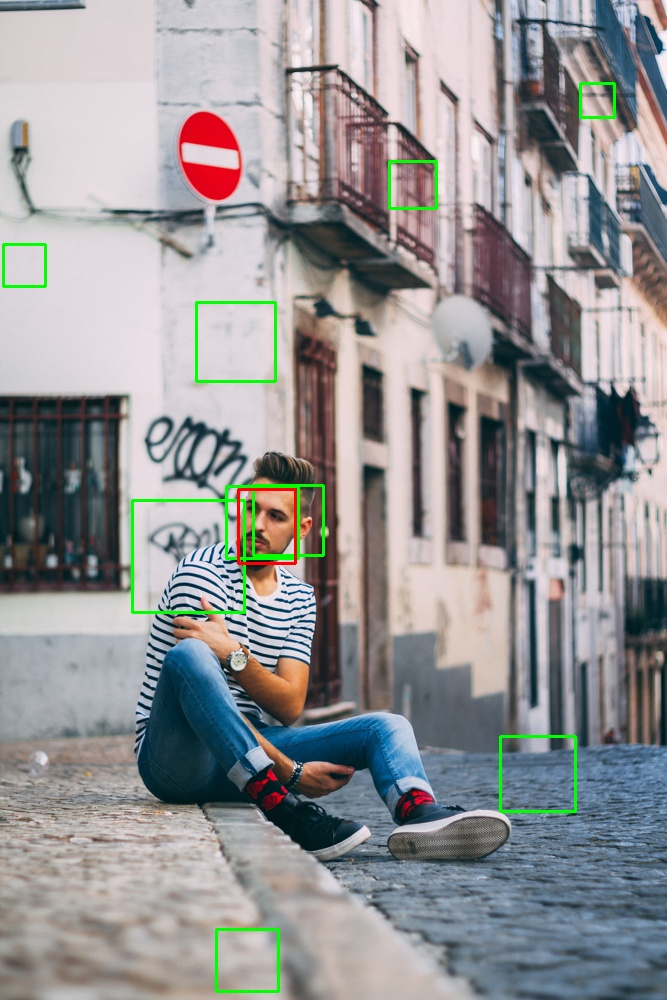
\includegraphics[height = 0.18\textheight]{images/NoEntry1.jpg}\label{fig:face1}}
  \hfill
  \subfloat[NoEntry5.jpg]{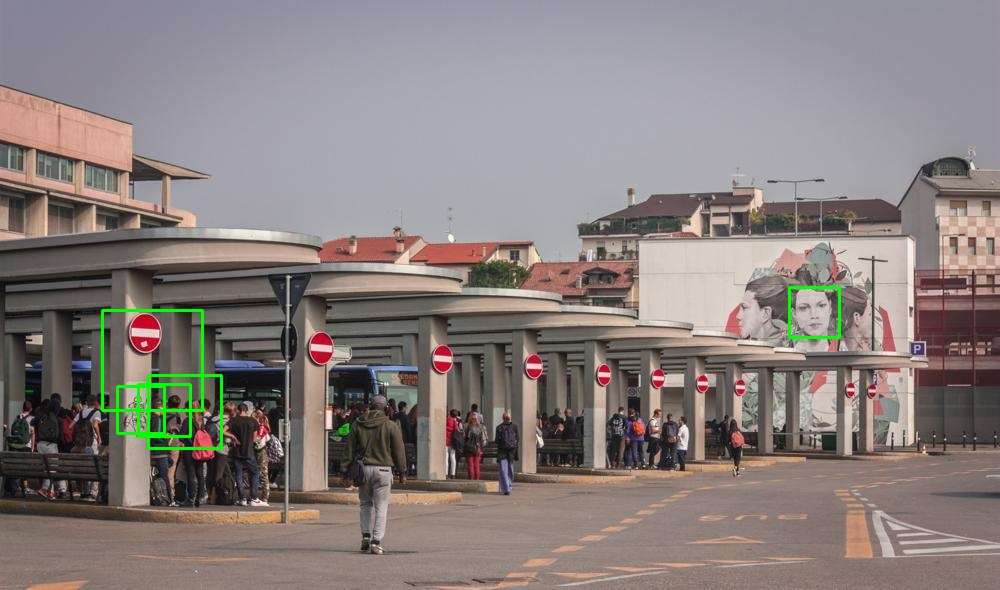
\includegraphics[height = 0.18\textheight]{images/NoEntry5.jpg}\label{fig:face5}}
  \hfill
  \subfloat[NoEntry11.jpg]{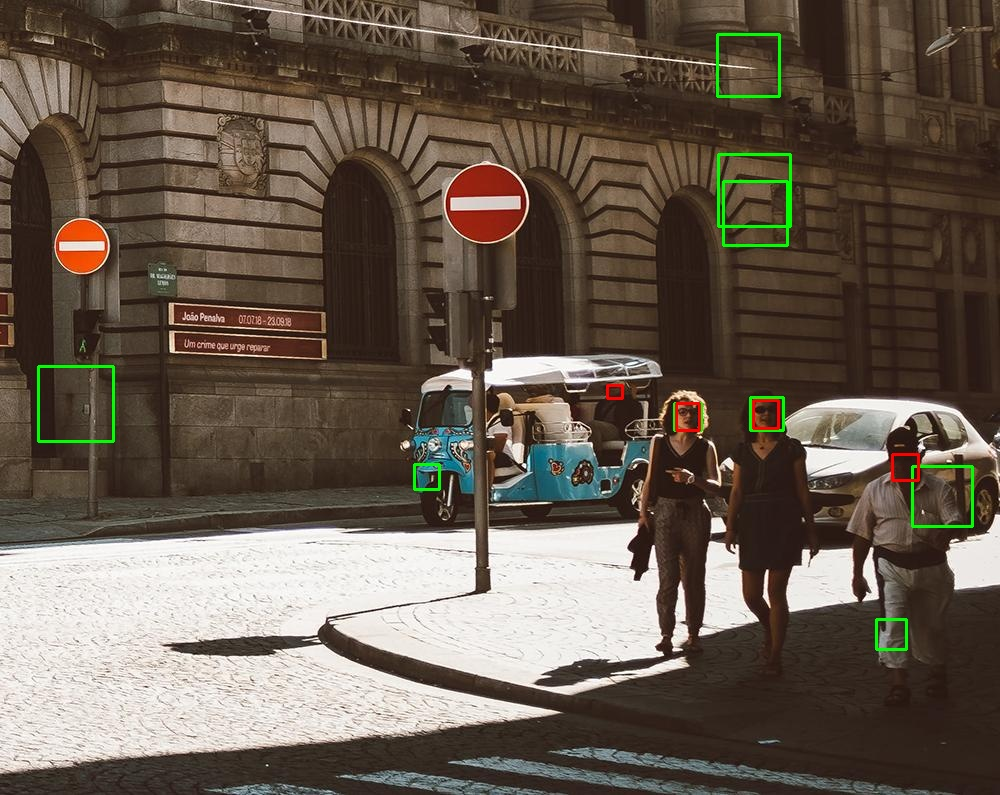
\includegraphics[height = 0.18\textheight]{images/NoEntry11.jpg}\label{fig:face11}}
  \hfill
  \subfloat[NoEntry2.jpg]{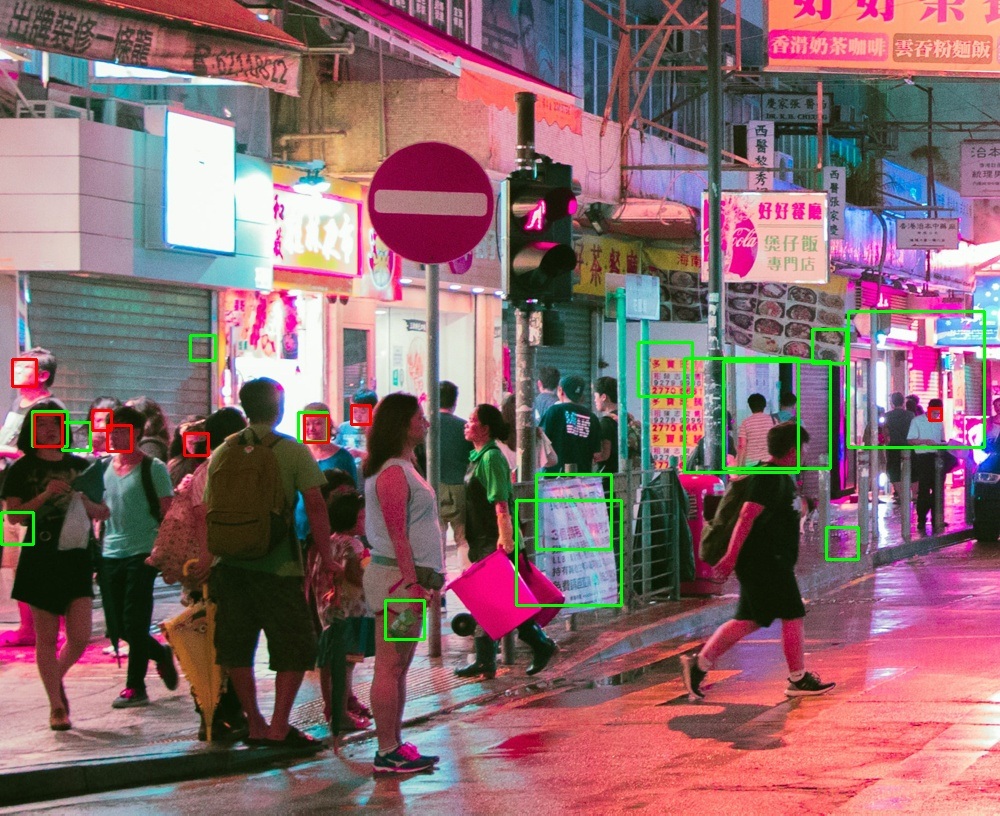
\includegraphics[height = 0.17\textheight]{images/NoEntry2.jpg}\label{fig:face2}}
  \hfill
  \subfloat[NoEntry4.jpg]{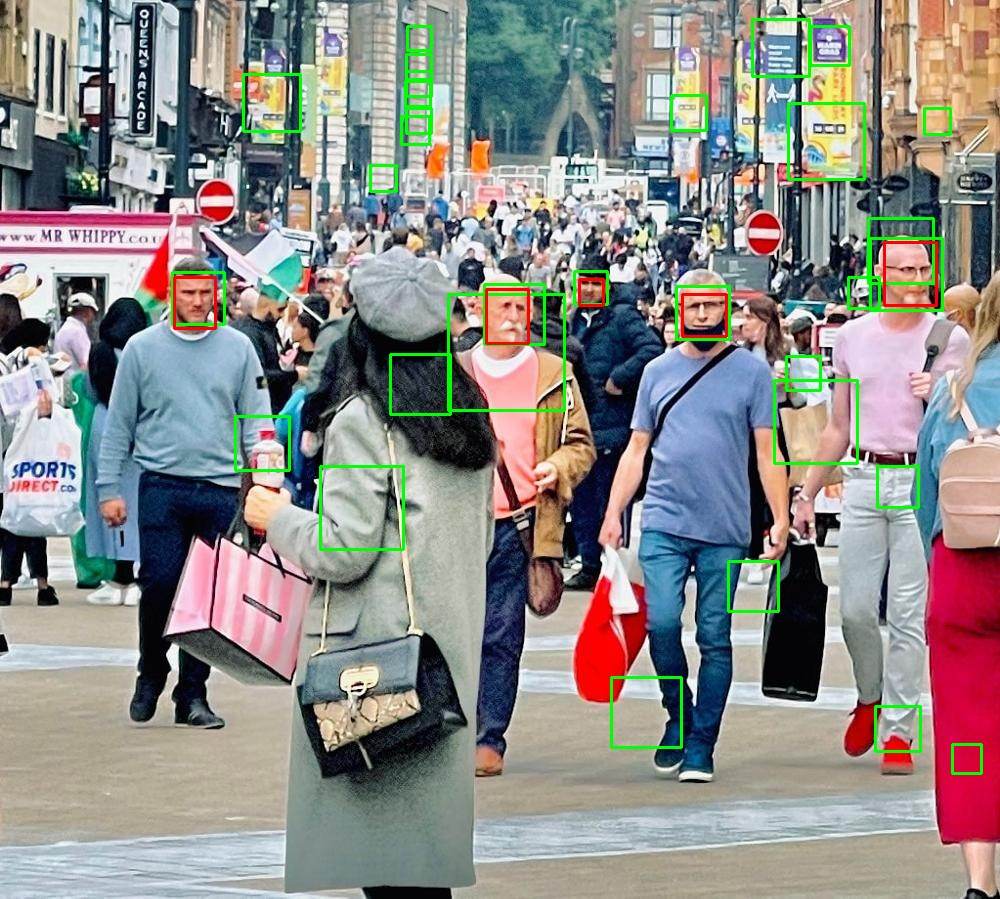
\includegraphics[height = 0.17\textheight]{images/NoEntry4.jpg}\label{fig:face4}}
  \hfill
  \subfloat[NoEntry7.jpg]{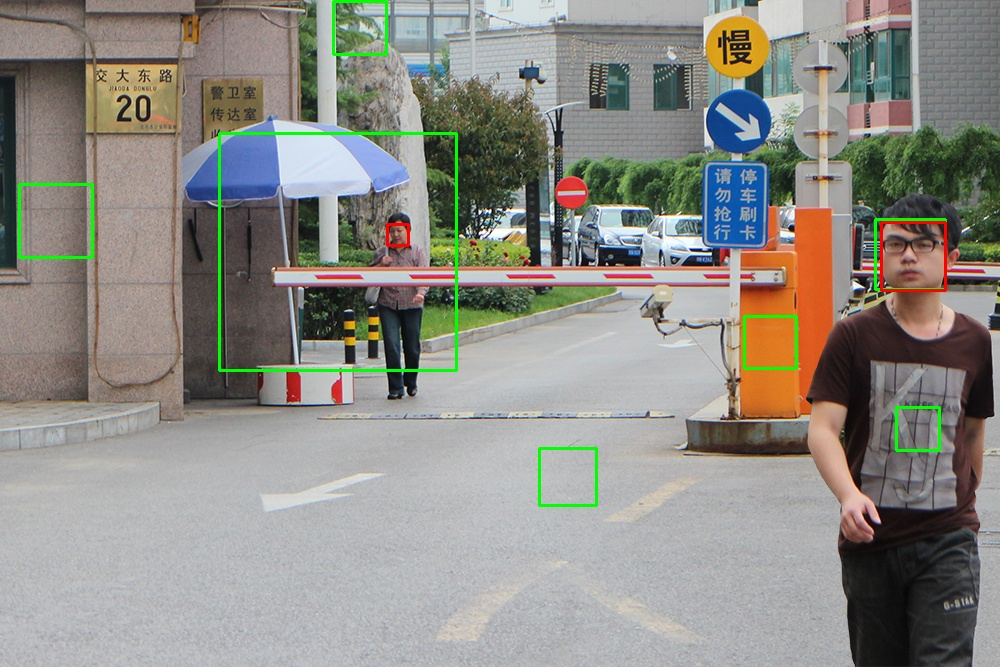
\includegraphics[height = 0.17\textheight]{images/NoEntry7.jpg}\label{fig:face7}}
  \caption{Six images with the bounding boxes of the ground truths (in red) and actually detected instances (in green) from the frontal face detector}\label{fig:face}
\end{figure}

\subsection{IOU, TPR and F\textsubscript{1} score}

\begin{table}[H]
  \begin{center}
    \caption{\label{tab:face}True positive rate and F\textsubscript{1} score of the frontal face detector on each image}
    \begin{tabular}{l l l} 
      \hline\hline
      Filename & True positive rate & F\textsubscript{1} score\\
      \hline
      NoEntry0.jpg & 0 & 0 \\ 
      NoEntry1.jpg & 0 & 0 \\ 
      NoEntry2.jpg & 0 & 0 \\ 
      NoEntry3.jpg & 0 & 0 \\ 
      NoEntry4.jpg & 0 & 0 \\ 
      NoEntry5.jpg & 0 & 0 \\ 
      NoEntry6.jpg & 0 & 0 \\ 
      NoEntry7.jpg & 0 & 0 \\ 
      NoEntry8.jpg & 0 & 0 \\ 
      NoEntry9.jpg & 0 & 0 \\ 
      NoEntry10.jpg & 0 & 0 \\ 
      NoEntry11.jpg & 0 & 0 \\ 
      NoEntry12.jpg & 0 & 0 \\ 
      NoEntry13.jpg & 0 & 0 \\ 
      NoEntry14.jpg & 0 & 0 \\ 
      NoEntry15.jpg & 0 & 0 \\ 
      \hline
    \end{tabular}
  \end{center}
\end{table}

\section{Building and testing my own detector}

\subsection{Training performance}

ROC graph
% \begin{tikzpicture}
% \begin{axis}[]
% \addplot+[
%   only marks,
%   % mark size=2.9pt
% ]
% table[]
% {fpr_tpr.dat};
% \end{axis}
% \end{tikzpicture}

\subsection{Testing performance}

\section{Integration with shape detectors}

\section{Improving my detector}



\clearpage
\begin{thebibliography}{9}
\end{thebibliography}
    

\end{document}